\documentclass[a4paper,12pt,twoside]{article}

\immediate\write18{echo -n "\\newcommand{\\gitroot}{" > gitroot.txt && git rev-parse --show-toplevel >> gitroot.txt && truncate -s-1 gitroot.txt && echo -n "}" >> gitroot.txt}

\input{gitroot.txt}
\usepackage{\gitroot/latexTemplate/preamble}


\newcommand{\Author}{Brandon Henke}
\newcommand{\course}{PHY831}
\newcommand{\professor}{Scott Bogner}

\newcommand{\mcols}{0}


\title{Homework 6}
\author{
	Brandon Henke\\
	\textit{\course}\\
	\textit{\professor}
}
\date{Novembre 14, 2021}


\fancyhead[LE,RO]{B. Henke}
\fancyhead[RE,LO]{\thepage}

\bibSetup{refs.bib}

\begin{document}
%\tableofcontents

\maketitle
\if\mcols1
\begin{multicols*}{2}
\fi

\setcounter{section}{6}
\subsection{}
\begin{align}
	PV\beta &= \log(Z) = g\sum_{\vb{p}}\log(\left(1-\eta e^{-\beta(\epsilon_p-\mu)}\right)^{-\eta}),\\
	P &= -\eta \frac{g}{V\beta} \sum_{\vb{p}} \log(1-\eta e^{-\beta(\epsilon-\mu)}), \quad (\epsilon_p = pc)\\
	&\approx -\eta \frac{g}{\beta} \int \frac{\dd[3]{p}}{(2\pi\hbar)^3} \log(1-\eta e^{-\beta(pc-\mu)}),\\
	&= \frac{4\pi g}{3(2\pi\hbar)^3} \int \dd{p}\frac{p^3 e^{-\beta(pc-\mu)}}{1-\eta e^{-\beta(pc-\mu)}},\\
	\mu = 0:\qquad&\\
	P &= \frac{4\pi g}{3(2\pi\hbar)^3} \int_0^\infty \dd{p}\frac{p^3 e^{-\beta pc}}{1-\eta e^{-\beta pc}},\\
	&= \left\{
		\begin{array}{rl}
			\frac{4\pi g}{3(2\pi\hbar)^3} \frac{1}{(\beta c)^4} \frac{\pi^4}{15}, & \eta = +1 \qq{(bosons)}\\
			\frac{4\pi g}{3(2\pi\hbar)^3} \frac{1}{(\beta c)^4} \frac{7\pi^4}{120}, & \eta = -1 \qq{(fermions)}
		\end{array}
	\right..
\end{align}
Hence:
\begin{equation}
	P = A g T^4,
\end{equation}
where
\begin{equation}
	A = \left\{
		\begin{array}{rl}
			\frac{4\pi}{3(2\pi\hbar)^3} \frac{k^4}{c^4} \frac{\pi^4}{15}, & \eta = +1 \qq{(bosons)}\\
			\frac{4\pi}{3(2\pi\hbar)^3} \frac{k^4}{c^4} \frac{7\pi^4}{120}, & \eta = -1 \qq{(fermions)}
		\end{array}
	\right..
\end{equation}\begin{align}
	\frac{E}{V} &= \frac{g}{V}\sum_{\vb{p}} \epsilon_p \ev{n_p}_\eta,\\
	&\approx g \int \frac{\dd[3]{p}}{(2\pi\hbar)^3} \frac{\epsilon_p}{e^{\beta(\epsilon_p-\mu)}-\eta},\\
	\mu = 0:\quad&\\
	\frac{E}{V} &= \frac{g4\pi c}{(2\pi\hbar)^3} \int \dd{p}\frac{p^3 e^{-\beta pc}}{1-\eta e^{-\beta pc}},\\
	&= \left\{
		\begin{array}{rl}
			\frac{g4\pi c}{(2\pi\hbar)^3} \frac{1}{(\beta c)^4} \frac{\pi^4}{15}, & \eta = +1\qq{(bosons)}\\
			\frac{g4\pi c}{(2\pi\hbar)^3} \frac{1}{(\beta c)^4} \frac{7\pi^4}{120}, & \eta = -1 \qq{(fermions)}
		\end{array}
	\right..
\end{align}
Hence:
\begin{equation}
	\frac{E}{V} = B g T^4,
\end{equation}
where $B = 3Ac$.

\subsection{}
\subsubsection{}
\begin{align}
	N_{\pm} &= \sum_{\vb{k}} \Theta(k_F^{\pm} - \abs{\vb{k}}),\\
	&\approx V\int \frac{\dd[3]{k}}{(2\pi)^3} \Theta(k_F^{\pm} - k),\\
	&= \frac{V}{2\pi} \frac{(k_F^\pm)^3}{6\pi^2}.\\
	\therefore k_F^\pm &= (6\pi^2 n_\pm)^{1/3},
\end{align}
where $n_\pm = N_\pm/V$.
\subsubsection{}
\begin{align}
	\ev{KE} &= \sum_{\vb{k}} \frac{\hbar^2 k^2}{2m} \Theta(k_F^+ - \abs{\vb{k}})
	+ \sum_{\vb{k}} \frac{\hbar^2 k^2}{2m} \Theta(k_F^- - \abs{\vb{k}}),\\
	&\approx V\int \frac{\dd[3]{k}}{(2\pi)^3} \frac{\hbar^2 k^2}{2m} \Theta(k_F^+ - \abs{\vb{k}})\nonumber\\
	&\ + V\int \frac{\dd[3]{k}}{(2\pi)^3} \frac{\hbar^2 k^2}{2m} \Theta(k_F^- - \abs{\vb{k}}),\\
	&= \frac{V}{2\pi^2} \frac{\hbar^2}{2m} \frac{((k_F^+)^5+(k_F^-)^5)}{5}.\\
	\rightarrow \frac{\ev{KE}}{V} &= \frac{\hbar^2}{4m\pi^2} \frac{((k_F^+)^5+(k_F^-)^5)}{5}.\\
	k_F^{\pm} = (6\pi^2n_{\pm})^{1/3}:\quad&\\
	\frac{\ev{KE}}{V} &= \frac{(6\pi^2)^{5/3}\hbar^2}{20m\pi^2} (n_+^5+n_-^5),\\
	&= \frac{3}{10m} \hbar^2 (6\pi^2)^{2/3} (n_+^{5/3}+n_-^{5/3}).
\end{align}
\subsubsection{}
For small deviations from the symmetric state ($n_\pm = n/2 \pm \delta$),
\begin{align}
	\frac{\ev{KE}}{V} &= \frac{3}{10m} \hbar^2 (6\pi^2)^{2/3} \left(\left(\frac{n}{2}+\delta\right)^{5/3}+\left( \frac{n}{2}-\delta \right)^{5/3}\right),\\
	&\approx \frac{6}{10m} \hbar^2 (6\pi^2)^{2/3} \left(
	\left(\frac{n}{2}\right)^{5/3}
	+ \frac{5}{9} \left(\frac{n}{2}\right)^{-1/3}\delta^2
	+ \frac{5}{243}\left(\frac{n}{2}\right)^{-7/3}\delta^4
	\right).
\end{align}
\subsubsection{}
\begin{align}
	\frac{U}{V} &= \alpha \left(\frac{n}{2}+\delta\right) \left(\frac{n}{2}-\delta\right),\\
	&= \alpha \frac{n^2}{4} - \alpha \delta^2.
\end{align}
Since $E = \ev{KE}+U$,
\begin{align}
	\frac{E}{V} &= \alpha \frac{n^2}{4} - \alpha \delta^2\nonumber\\
	&\ + \frac{6}{10m} \hbar^2 (6\pi^2)^{2/3} \left(
	\left(\frac{n}{2}\right)^{5/3}
	+ \frac{5}{9} \left(\frac{n}{2}\right)^{-1/3}\delta^2
	+ \frac{5}{243}\left(\frac{n}{2}\right)^{-7/3}\delta^4
	\right),\\
	&= \left(\frac{E}{V}\right)_{\delta=0} + \left( \frac{4}{3}(3\pi^2)^{2/3}\frac{\hbar^2}{2m} n^{-1/3}-\alpha \right)\delta^2 + \mathcal{O}(\delta^4).\\
	\therefore \alpha &> \alpha_c = \frac{4}{3}(3\pi^2)^{2/3}\frac{\hbar^2}{2m} n^{-1/3}
\end{align}
causes the electron gas to have the ability to lower its energy by developing a magnetization.
\subsubsection{}
\begin{figure}[H]
	\centering
	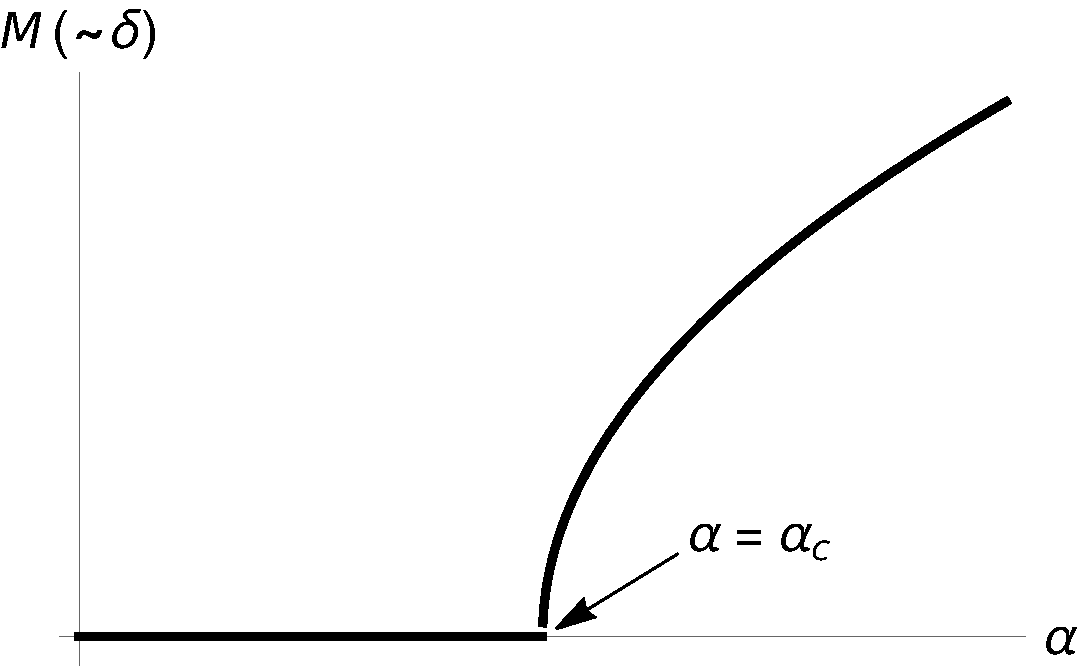
\includegraphics[width=0.6\textwidth]{figures/2eFig.pdf}
	\caption{}
	\label{fig: 2e graph}
\end{figure}
The magnetization starts at $0$ for $\alpha < \alpha_c$, but, for $\alpha \geq \alpha_c$, the magnetization (which is essentially the quantity $\delta$) grows as $\sqrt{a-a_c}$.
\subsection{}
\subsubsection{}
\begin{align}
	\mathscr{G} &= -\frac{1}{\beta} \log(\mathscr{Z}),\\
	&= \frac{\eta}{\beta} \sum_{\vb{p}} \log(1-\eta e^{-\beta(\epsilon_p - \mu)}),\\
	&= \frac{\eta}{\beta} V \int \frac{\dd[D]{p}}{(2\pi\hbar)^D} \log(1-\eta e^{-\beta(\epsilon_p - \mu)}),\\
	&= \frac{\eta V}{(2\pi\hbar)^D \beta} S_D \int \dd{p} p^{D-1} \log(1-\eta e^{-\beta(\epsilon_p - \mu)}), \qquad \left(S_D = \int \dd{\Omega_D}\right)\\
	&\qquad\vdots \qquad(\text{Mathematica})\nonumber\\
	\mathscr{G} &= -\frac{VS_D\alpha s}{(2\pi\hbar)^D D} \int \dd{p}p^{D+s-1} \frac{e^{-\beta(\alpha p^s - \mu)}}{1-\eta e^{-\beta(\alpha p^s - \mu)}}.
\end{align}
Let $x = \beta\alpha p^s$:
\begin{align}
	\mathscr{G} &= -\frac{VS_D\alpha s}{(2\pi\hbar)^D D} \frac{1}{s\beta\alpha} \left(\frac{1}{\beta\alpha}\right)^{D/s} \int \dd{x} \frac{x^{D/s}} {\mathcal{z}^{-1}e^x-\eta},\\
	&= -\frac{VS_D \alpha}{(2\pi\hbar)^D D} \left(\frac{1}{\beta \alpha}\right)^{D/s+1} \Gamma\left(\frac{D}{s}+1\right) f_{\frac{D}{s}+1}^\eta(\mathcal{z}).
\end{align}
For the following, $V = L^D$.
\begin{align}
	n &= \frac{N}{V},\\
	&= \frac{1}{V} \sum_{\vb{p}} \frac{1}{\mathcal{z}e^{\beta\epsilon_p} - \eta},\\
	&= \int \frac{\dd[D]p}{(2\pi\hbar)^D} \frac{1}{\mathcal{z}e^{\beta\alpha p^s}-\eta},\\
	&= \frac{S_D}{(2\pi\hbar)^D}\int \dd{p}p^{D-1} \frac{1}{\mathcal{z}e^{\beta\alpha p^s}-\eta},\\
	&\qquad\vdots \qquad\text{(Same integral as before)}\\
	&= \frac{S_D}{(2\pi\hbar)^D} \frac{1}{s} \frac{1}{\beta\alpha}^{D/s} \Gamma\left(\frac{D}{s}\right) f_{\frac{D}{s}}^\eta(\mathcal{z}).
\end{align}
\subsubsection{}
\begin{align}
	PV &= -\mathscr{G}.\\
	E &= -\pdv{\beta}\log{\mathscr{Z}}\mid_{\mathcal{z} = \text{const.}},\\
	&= \frac{D}{s} \mathscr{G}.\\
	\frac{PV}{E} &= \frac{s}{D}.
\end{align}
\subsubsection{}
As $T\rightarrow 0$,
\begin{equation}
	\lim_{T\rightarrow 0} \frac{1}{e^{\beta(\epsilon_p-\mu)}+1} = \Theta(\epsilon_p - \mu).
\end{equation}
Itaque,
\begin{align}
	\frac{E}{V} &= \frac{1}{V} \sum_{\vb{p}} \alpha p^s \Theta(p_f-p),\\
	&= \int \frac{\dd[D]{p}}{(2\pi\hbar)^D} \alpha p^s,\\
	&= \frac{S_d\alpha}{(2\pi\hbar)^D} \frac{p_F^{D+s}}{D+s}.\\
	n &= \int \frac{\dd[D]{p}}{(2\pi\hbar)^D} \Theta(p_F - p).\\
	p_F &= \left(\frac{(2\pi\hbar)^D D}{S_D} n\right)^{1/D}.\\
	\therefore
	\frac{E}{V} &= \frac{S_D\alpha}{(2\pi\hbar)^D} \frac{\left(\frac{(2\pi\hbar)^D D}{S_D} n\right)^{1+(s/D)}}{D+s},\\
	\frac{E}{V} &\propto n^{1+(s/D)}.
\end{align}
\begin{align}
	\frac{PV}{E} &= \frac{s}{D},\\
	P &= \frac{s}{D}\frac{S_D\alpha}{(2\pi\hbar)^D} \frac{\left(\frac{(2\pi\hbar)^D D}{S_D} n\right)^{1+(s/D)}}{D+s},\\
	P &\propto n^{1+(s/D)}.
\end{align}
\subsubsection{}
If, in the limit $\mathcal{z} \rightarrow 1$, $f_{D/s}^+(\mathcal{z} \rightarrow 1)$ is not finite, then no Bose-Einstein condensation forms.
However, if $f_{D/s}^+(\mathcal{z} \rightarrow 1)$ is finite, then Bose-Einstein condensation forms.

The fugacity at $\mathcal{z} = 1$ is given by
\begin{align}
	f_{D/s}^+(\mathcal{z}=1) &= \lim_{\varepsilon \rightarrow\infty} \frac{1}{\Gamma\left(\frac{D}{s}\right)} \int_0^\varepsilon \dd{x} \frac{x^{(D/s)-1}}{e^x-1},\\
	&= \lim_{\varepsilon \rightarrow\infty}\frac{1}{\Gamma\left(\frac{D}{s}\right)} \int_0^\varepsilon \dd{x} x^{(D/s)-1} \left(x+\frac{x^2}{2!} + \dots\right)^{-1},\\
	&\approx \lim_{\varepsilon \rightarrow\infty} \frac{1}{\Gamma\left(\frac{D}{s}\right)} \int_0^\varepsilon \dd{x} x^{(D/s)-2}.
\end{align}
This converges for $0 > (D/s)-2 > -1$, so if $D > s$ a Bose-Einstein condensate can form.
Therefore, if $D = s = 2$ no Bose-Einstein condensate will form.

\subsection{}


\printBib


\if\mcols1
\end{multicols*}
\fi
\end{document}
